\documentclass[a4paper,11pt]{article}
\input{/home/tof/Documents/Cozy/latex-include/preambule_lua.tex}
\newcommand{\showprof}{show them}  % comment this line if you don't want to see todo environment
\fancyhead[L]{Processus et ordonnancement}
\newdate{madate}{10}{09}{2020}
\fancyhead[R]{Terminale - NSI} %\today
\fancyfoot[L]{~\\Christophe Viroulaud}
\fancyfoot[C]{\textbf{Page \thepage}}
\fancyfoot[R]{\includegraphics[width=2cm,align=t]{/home/tof/Documents/Cozy/latex-include/cc.png}}

\begin{document}
\begin{Form}
\section{Problématique}
Un processeur ne peut exécuter qu'une seule instruction à la fois. Pourtant sur un ordinateur, il est possible d'écouter de la musique tout en surfant sur le web.
\begin{center}
\shadowbox{\parbox{12cm}{\centering Comment réaliser plusieurs activités en même temps sur une machine?}}
\end{center}
\section{Les processus}
\subsection{Définition}
Nous travaillerons sur un système de type \emph{Unix}. La page ci-après
\begin{center}
\url{https://tinyurl.com/y839kd4f}
\end{center}
propose un simulateur d'un \emph{terminal} Linux.\\
Un \emph{programme} est un fichier en mémoire qui ne fait rien. Un \emph{processus} est l'exécution d'un programme. Il est possible de visualiser les processus en cours exécution en utilisant la commande \textbf{top} (figure \ref{top}).
\begin{figure}[!h]
\centering
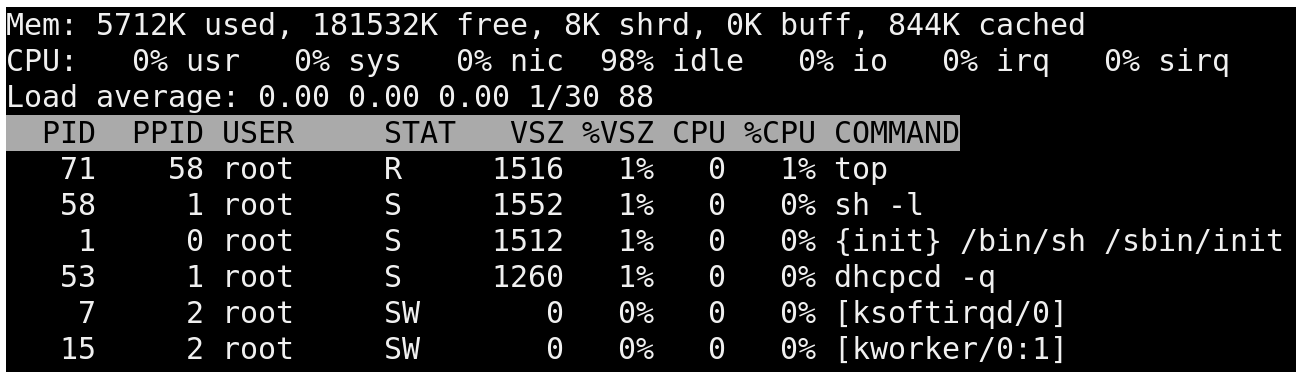
\includegraphics[width=10cm]{ressources/top.png}
\captionof{figure}{Processus en cours}
\label{top}
\end{figure}
Nous pouvons comparer cette commande au \emph{gestionnaire de tâches} de Windows.
\subsection{Création d'un processus}
Chaque processus possède un identifiant unique, \emph{le PID}. Au démarrage de la machine un premier processus spécial  (\emph{init}) est lancé. Ce processus crée d'autres \emph{processus fils}. Ainsi chaque processus possède un (seul) parent, \emph{le PPID}.\\
La commande
\begin{lstlisting}
ps sort=pid
\end{lstlisting}
liste la totalité des processus.\\
Il est possible de tuer un processus en appelant l'instruction:
\begin{lstlisting}
kill numéro_PID
\end{lstlisting}
\begin{commentprof}
d'autres infos: nom de l'utilisateur qui a crée, utilisation CPU, état (STAT):
\begin{itemize}
\item R en cours d'exécution.
\item T processus stoppé.
\item I processus endormi (>20s).
\item S processus endormi (<20s).
\item Z processus zombie.
\item D processus non interruptible.
\item W processus swappé (échangé) sur disque. 
\end{itemize}
\end{commentprof}
\section{Ordonnancement}
\subsection{Le chef d'orchestre}
Dans le système plusieurs processus sont en cours simultanément, mais le processeur ne peut exécuter qu’une seule instruction à la fois. Le processeur travaille donc \emph{en temps partagé}. Il bascule constamment d’un processus à l’autre.\\
\begin{commentprof}
chaque processus considère qu'il a le processeur pour lui tout seul. multiprogrammation\\
scheduleur = 1 module du système d'exploitation
\end{commentprof}
\emph{L'ordonnanceur (scheduleur)} sélectionne le prochain processus prêt (\emph{Ready}) qui sera exécuté par le processeur. L'objectif est d'obtenir un \emph{temps de traitement moyen} le plus court possible.
\subsection{Le scheduling}
Les algorithmes d’ordonnancement peuvent être classés en deux catégories:
\begin{itemize}
\item \textbf{Non pré~emptif:} Sélectionne un processus, puis le laisse s’exécuter jusqu’à ce qu’il bloque (soit sur une E/S, soit en attente d’un autre processus) où qu’il libère volontairement le processeur.
\item \textbf{Pré~emptif:} Sélectionne un processus et le laisse s’exécuter pendant un délai déterminé.
\end{itemize}
\subsection{Quelques algorithmes d'ordonnancement}
\subsubsection{First Come First Served}
\begin{commentprof}
FIFO
\end{commentprof}
Une fois que la CPU a été allouée à un processus, celui-ci garde la CPU jusqu’à ce qu’il la libère. Cet algorithme est particulièrement incommode pour le temps partagé où il est important que chaque utilisateur obtienne la CPU à des intervalles réguliers.
\subsubsection{Shortest Job First}
Quand la CPU est disponible, elle est assignée au processus qui possède le prochain cycle le plus petit. La difficulté est pouvoir connaître la longueur de la prochaine requête de la CPU.
\begin{commentprof}
 Si deux processus possèdent la même longueur, le FCFS est utilisé.
\end{commentprof}
\subsubsection{Round Robin}
Chaque processus a une petite unité de temps appelée \emph{quantum} (en général de 10 à 100 ms). L'ordonnanceur parcourt la file d’attente des processus prêts et alloue la CPU à chaque processus pendant un quantum. La performance du \emph{tourniquet} dépend fortement du choix du quantum de base. 
\begin{commentprof}
Linux offre trois politiques d'ordonnancement (les 3 cités). Un système de priorité est également mis en place. Par défaut, un processus est associé à la politique de temps partagé. Seul root peut associer un processus à une des classes d’ordonnancement en temps réel.
\end{commentprof}
\end{Form}
\end{document}